\subsection{Winkelrichtgröße und Eigenträgheitsmoment der Drillachse}
\begin{table}[h!]
	\begin{center}
		\begin{tabular}{cc}
			Anodenspannung [V] & Anodenstrom [mA]\\ \hline
			10	&0,044\\
			20	&0,088\\
			30	&0,108\\
			40	&0,119\\
			50	&0,126\\
			60	&0,128\\
			70	&0,132\\
			80	&0,135\\
			90	&0,138\\
			100	&0,141\\
			110	&0,144\\
			120	&0,146\\
			130	&0,147\\
			140	&0,149\\
			150	&0,150\\
			160	&0,151\\
			170	&0,152\\
			180	&0,154\\
			190	&0,155\\
			200	&0,156\\
			210	&0,157
		\end{tabular}
		\caption{Kennlinie 1 (Heizwerte: 4,2V; 2,1A)}
		\label{taba1}
	\end{center}
\end{table}
Zur Bestimmung der Winkelrichtgröße wird für jedes Wertepaar die Winkelrichtgröße $D=\frac{F*r}{\varphi}$ bestimmt. Siehe Tabelle \ref{tab:drillachse}. Als Mittelwert ergibt sich
\begin{align*}
D=(5,642\pm1,247)*10^{-4}\frac{F*r}{\varphi}
\end{align*}
\\
\\
\begin{table}[h]
	\begin{center}
		\begin{tabular}{cccc}
Abstand $a+0,014$&Periodendauert $T*3$&Abstand $a^2$&Periodendauer $T^2$\\ \hline

0,0438&6,32&0,00088804&4,438\\
0,06&6,81&0,002116&5,1529\\
0,08&7,86&0,004356&6,8644\\
0,1&8,6&0,007396&8,21777778\\
0,12&9,84&0,011236&10,7584\\
0,14&10,8&0,015876&12,96\\
0,16&12,3&0,021316&16,81\\
0,18&13,5&0,027556&20,25\\
0,2&14,66&0,034596&23,879511\\
0,22&16,35&0,042436&29,7025

			\end{tabular}
		\caption{Werte zur Bestimmung des Eigenträgheitsmomentes}
		\label{tab:eigentragheitsmom}
	\end{center}
\end{table}
	\begin{figure}[h]
		\begin{center}
		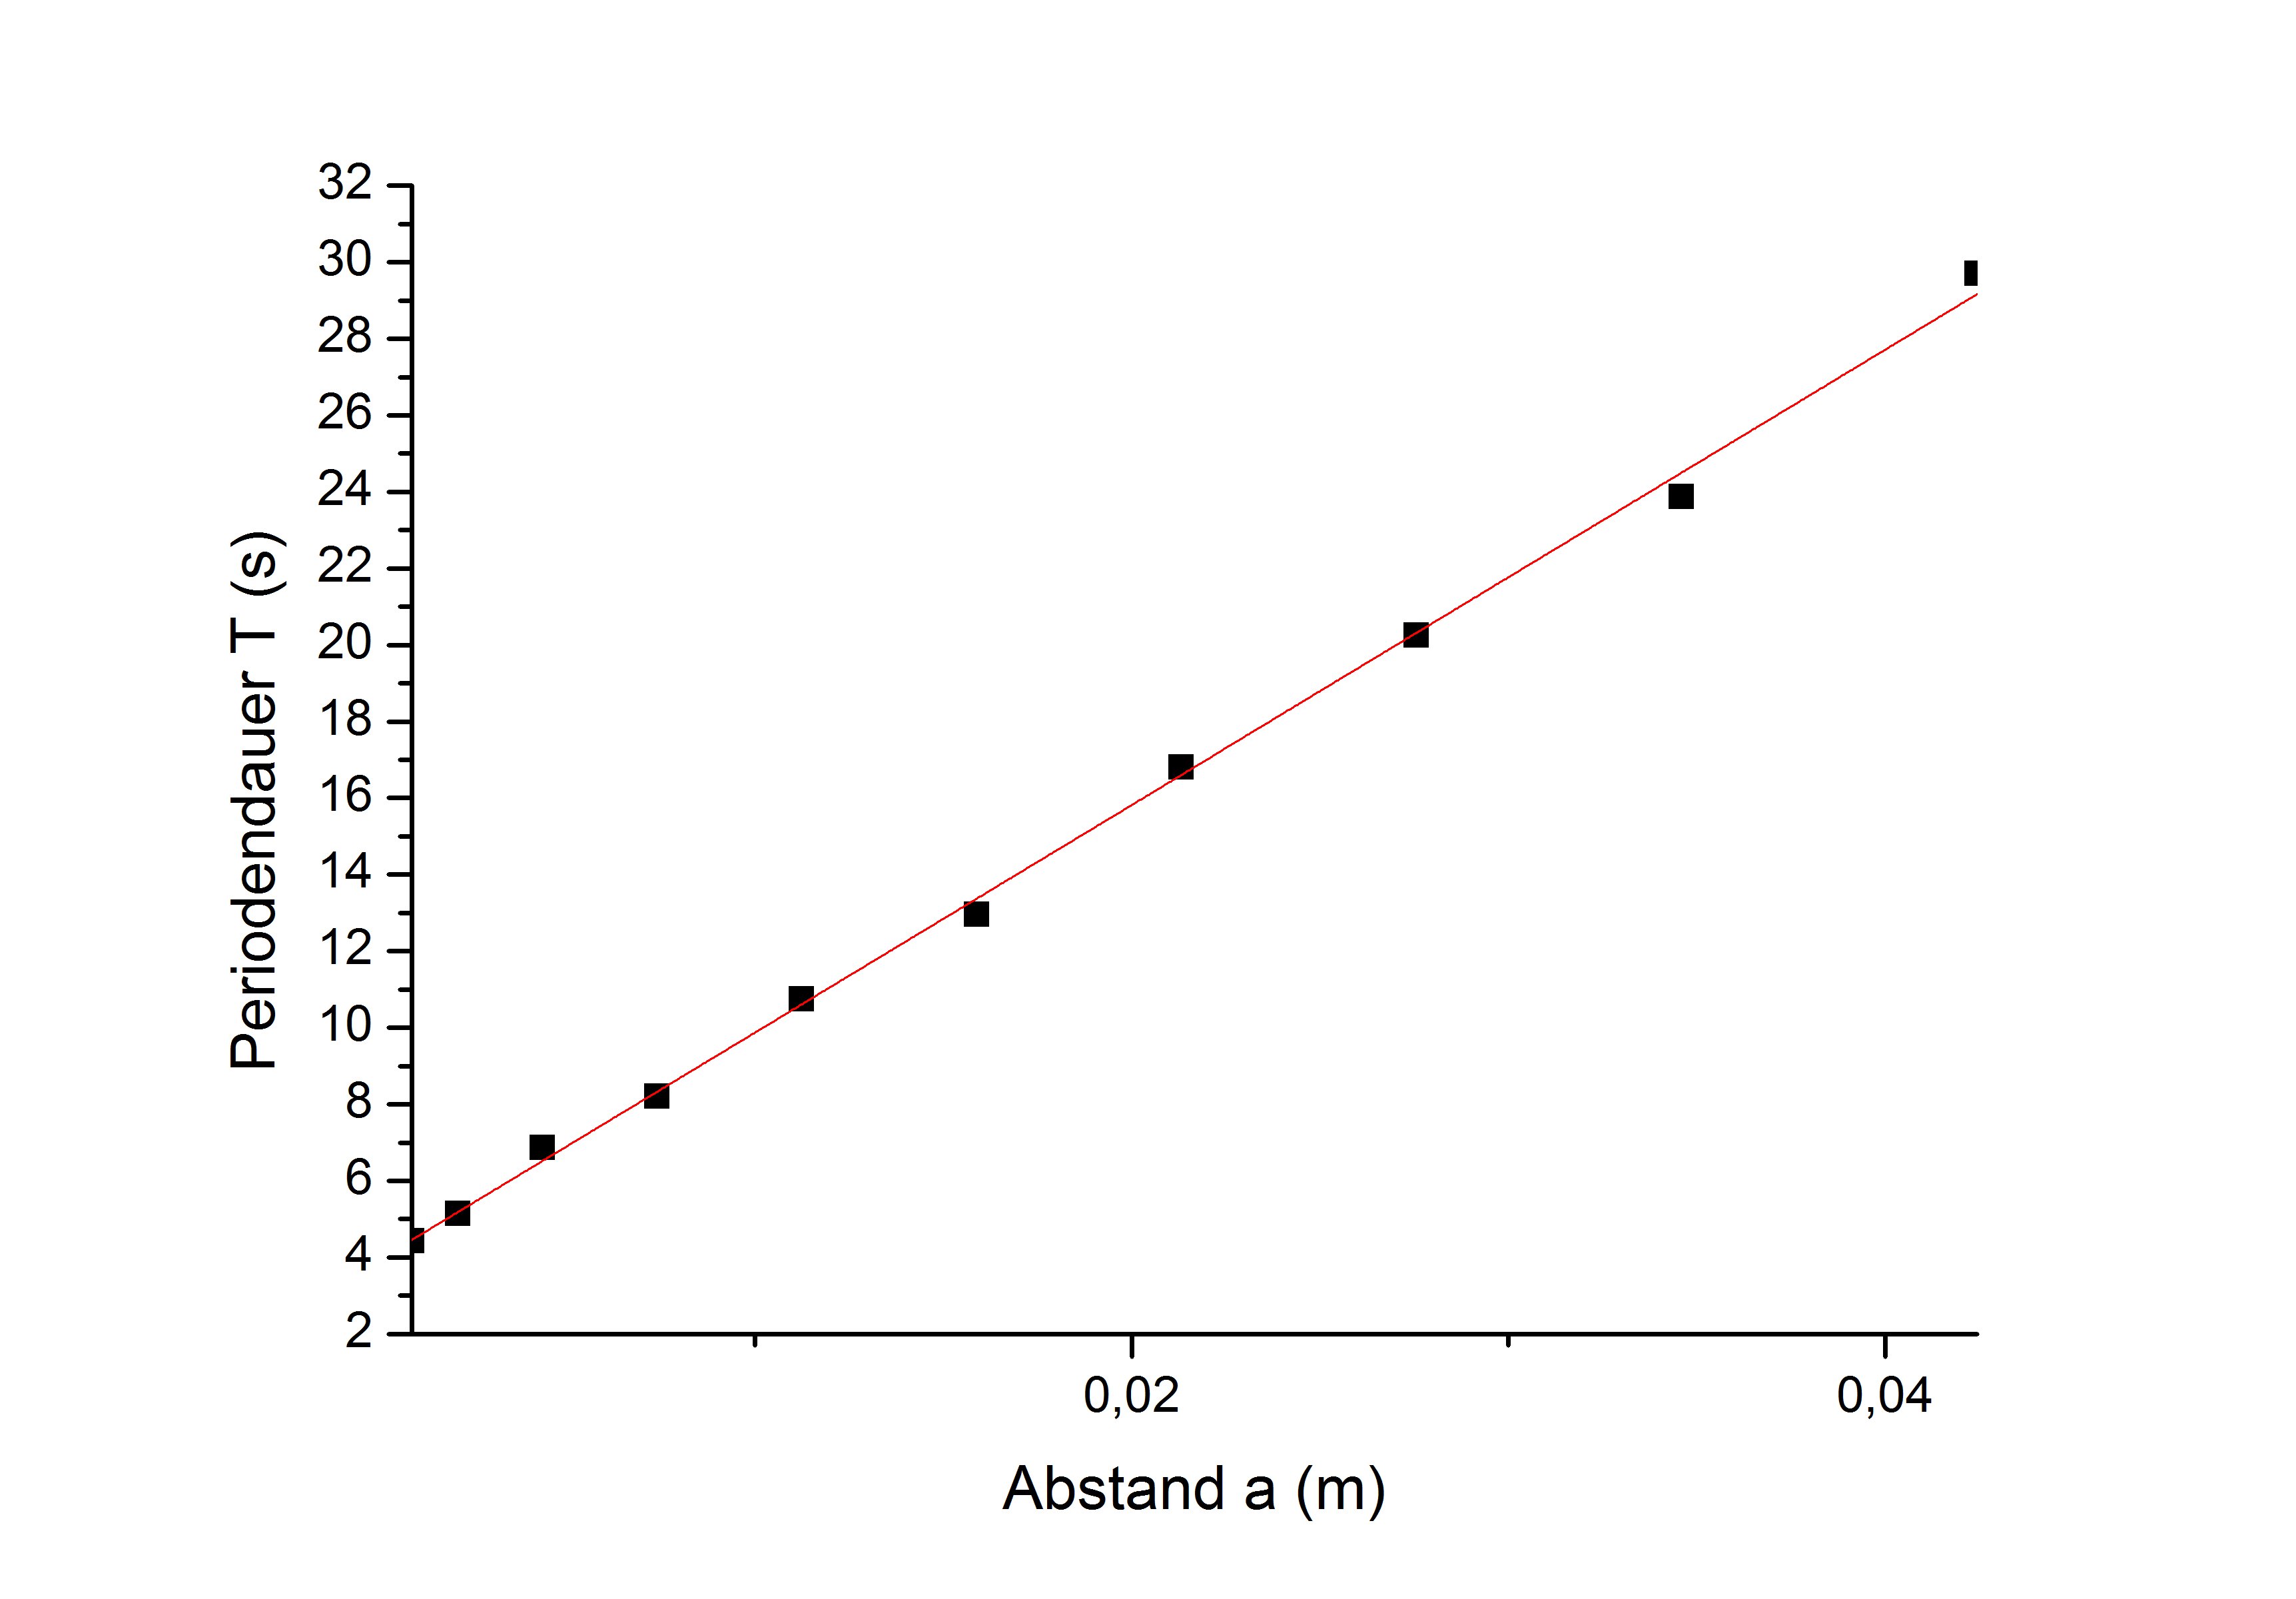
\includegraphics[scale=0.3]{eigentragmom.jpg}
		\caption{Graphische Bestimmung des Eigenträgheitsmoment}
		\label{pic:eigentragmom}
		\end{center}	
	\end{figure}
Das Eigenträgheitsmoment der Drillachse wird Graphisch bestimmt. Dazu wird $T^2$ gegen $a^2$ (Tab. \ref{tab:eigentragheitsmom}) aufgetragen. 
Aus Graphik \ref{pic:eigentragmom} ergibt sich ein y-Achsen Schnitt bei $y(0)=3,926\pm0,181$.


Aus Gleichung \ref{} und dem Steinerschen Satz \ref{} lässt sich das Trägheitsmoment bestimmen
\begin{align}
I_{DS}=\frac{T^2*D}{4\pi^2}=(5,611\pm1,268)*10^{-5}kgm^2
\end{align}

In $I_{DS}$ ist allerdings nicht nur das Trägheitsmoment der Drillachse, sondern auch das, des Stabes enthalten. Dieses lässt sich nach \ref{} berechenen und von $I_{SD}$ abziehen. Mit m=96,3g und l=60cm ergibt sich
\begin{align}
I_{D}=I_{DS}-I_{St}=I_{DS}-\frac{ml^2}{12}=(-2,833\pm0,013)*10^{-3}kg*m^2
\end{align}
als Eigendrehmoment der Drillachse.
\\
\\
\subsection{Trägheitsmoment einer Kugel und eines Zylinders}
\begin{table}[h]
	\begin{center}
		\begin{tabular}{cc|ccc}
			Brückenspannung $U_B$ [mV]&$\chi_{U}*10^-3$ & $\Delta R$ [m$\Omega$]&$R_3[\text{m}\Omega]$&$\chi_R*10^{-3}$\\ \hline
			3,5	&4,493&140&2555&3,165\\
			2,8	&3,594&90&2552&2,037\\
			3	&3,851&100&2550&2,265\\
			3,7	&4,750&155&2600&3,444
		\end{tabular}
		\caption{$Nd_2O_3$}
		\label{tab2}
	\end{center}
\end{table}
